\documentclass[../qm.tex]{subfiles}
\begin{document}
	In this appendix, we give the table of Clebsch-Gordan coefficients used in the addition of angular momenta, in order to switch from a common basis between $\opr{J}^2_1,\opr{J}^2_2,\opr{J}_{z1},\opr{J}_{z2}$ to the new ``total'' common basis of $\opr{J}^2_1,\opr{J}^2_2,\opr{J}^2,\opr{J}_z$, where the total angular momentum operator is defined as follows
	\begin{equation}
		\begin{aligned}
			\vecopr{J}&=\vecopr{J}_1\otimes\1+\1\otimes\vecopr{J}_2\\
			\opr{J}_z&=\opr{J}_{z1}\otimes\1+\1\otimes\opr{J}_{z2}\\
			\opr{J}^2&=\left( \vecopr{J}_1\otimes\1+\1\otimes\vecopr{J}_2 \right)^2
		\end{aligned}
		\label{eq:cgcoeffputt}
	\end{equation}
	Its eigenvalues are the following
	\begin{equation}
		\begin{aligned}
			\opr{J}^2\ket{j_1,j_2,j,m}&=\hbar^2j(j+1)\ket{j_1,j_2,j,m}\\
			\opr{J}_z\ket{j_1,j_2,j,m}&=\hbar m\ket{j_1,j_2,j,m}
		\end{aligned}
		\label{eq:jsqeigenvalputt}
	\end{equation}
	And are subject to the following constraints
	\begin{equation}
		\begin{aligned}
			m&=m_1+m_2,\quad-j\le m\le j\\
			0&\le\abs{j_1-j_2}\le j\le j_1+j_2
		\end{aligned}
		\label{eq:eigenvaltotangmom}
	\end{equation}
	\newpage
	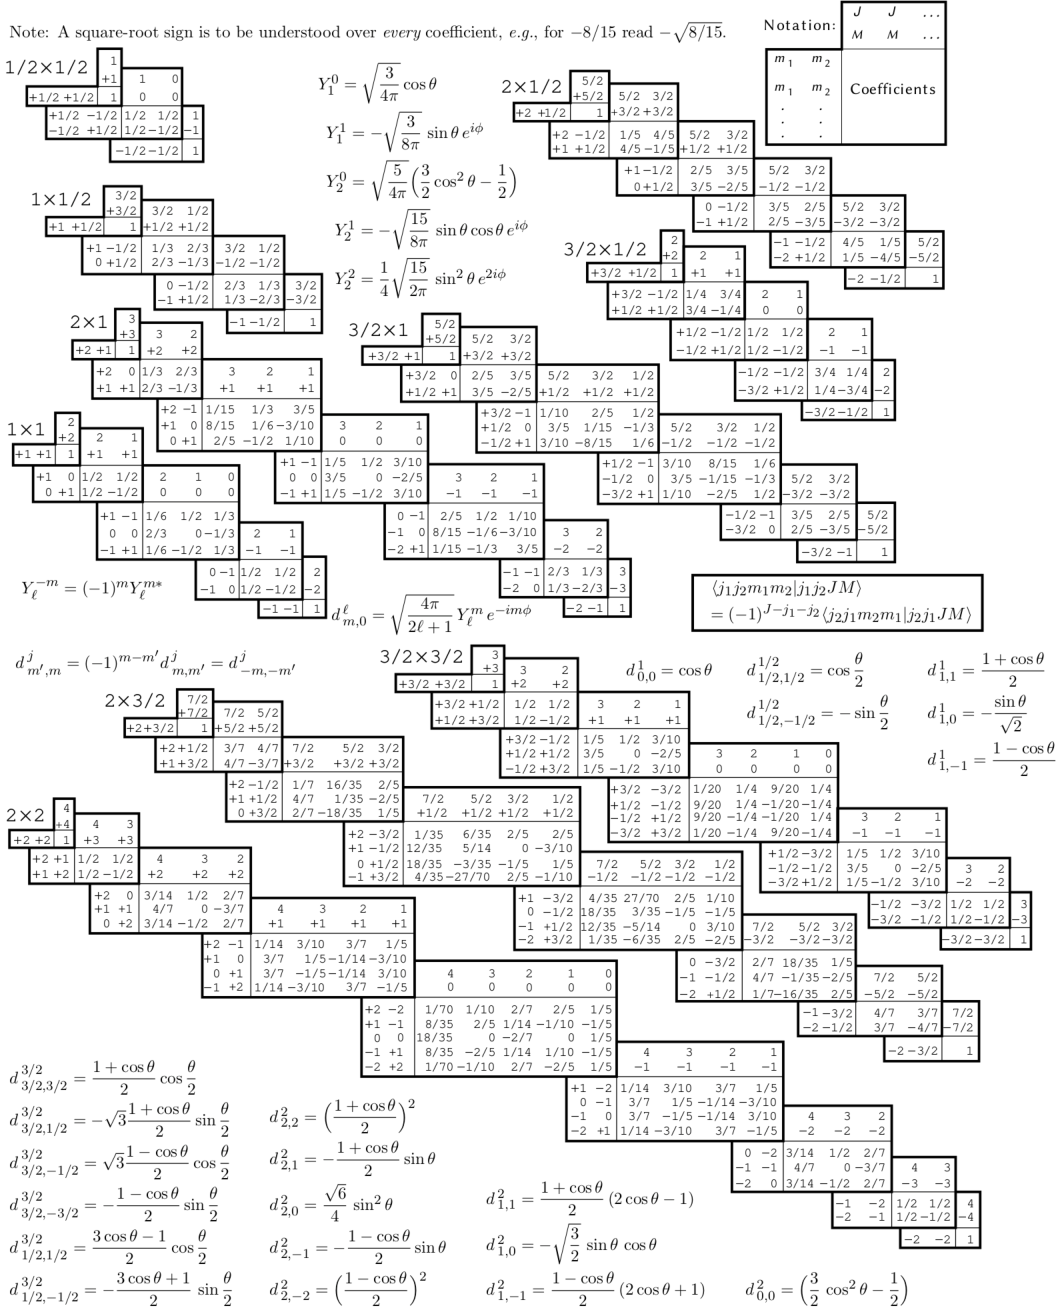
\includegraphics[width=\textwidth,height=\textheight]{clebschgordan1.pdf}
\end{document}
